W tej części rozprawy analizowany jest wpływ parametrów środowiskowych na ocenę bazową CVSS, a tym samym na możliwości zmiany kategorii krytyczności podatności, na przykład z kategorii niskiej na krytyczną. Możliwość zmiany kategorii krytyczności podatności z niskiej na krytyczną pozwala na stwierdzenie mówiące o ryzyku nienaprawienia podatności z niedoszacowaną oceną lub naprawienia podatności z przeszacowaną oceną za pomocą modeli zarządzania podatnościami wykorzystującymi ocenę bazową CVSS (Rysunek \ref{fig:chapter1:vm-model-cvss2}, \ref{fig:chapter1:vm-model-cvss3}). W związku z tym, że wykrywane jest coraz więcej podatności w środowiskach teleinformatycznych, istnieje możliwość, że podatność niedoszacowana, posiadająca klasyfikacje niską, nigdy nie zostanie naprawiona przez administratorów, ponieważ podatności o wyższej klasyfikacji zawsze będą naprawiane w pierwszej kolejności. W konsekwencji nienaprawiona podatność niedoszacowana o klasyfikacji niskiej, która w rzeczywistości mająca klasyfikację na przykład średnią wpływa na czas ekspozycji podatności w systemie, która może zostać wykorzystana przez atakującego. Należy jednak pamiętać, że wpływ parametrów środowiskowych CVSS może nie być brany pod uwagę w procesie napraw podatności w przypadku małych organizacji, gdzie liczba skanowanych zasobów i wykrytych podatności jest niewielka. Natomiast w każdej organizacji osoba odpowiedzialna za proces zarządzania podatnościami musi podjąć decyzję czy uważa, że jego organizacja wymaga usprawnień w postaci uwzględniania parametrów środowiskowych CVSS.

\bigbreak
Do przeprowadzenia analizy wybrano po jednej podatności reprezentującej każdą klasyfikację krytyczności według oceny bazowej dla standardu CVSS 2.0 (Tabela \ref{tab:cvss_criticality_2}) oraz 3.x (Tabela \ref{tab:cvss_criticality_3}). Wybrane podatności zostały wykryte w środowisku teleinformatycznym A za pomocą oprogramowania skanującego Nessus. Dla każdej kategorii krytyczności wyniki analizy uporządkowano w następujący sposób. Najpierw porównano wpływ parametrów środowiskowych na ocenę bazową CVSS 2.0. W tym celu napisany został program, za pomocą którego obliczono wszystkie możliwe do uzyskania wartości oceny środowiskowej CVSS 2.0 dla każdej kombinacji parametrów środowiskowych $CIA$, $TD$, $CDP$ (Załącznik Z1), a następnie przeanalizowano liczbę oraz zakres zmian w kategoriach podatności. Wzięto pod uwagę wadę oceny środowiskowej CVSS 2.0 dotyczącej parametru $TD$, który służy do ustalania liczby systemów wrażliwych na daną podatność, przez co znacząco zaniża oceny wszystkich wykrytych podatności. Dlatego też w dalszej części dokonano analizy wpływu parametrów środowiskowych na ocenę bazową CVSS 3.x. W tym celu również został napisany program, za pomocą którego obliczono wszystkie możliwe do uzyskania wartości oceny środowiskowej CVSS 3.x dla każdej możliwej kombinacji parametrów środowiskowych $CIA$ (Załącznik Z2). Następnie ponownie przeanalizowano liczbę oraz zakres zmian w kategoriach podatności. Otrzymane wyniki pozwoliły na wyciągnięcie istotnych wniosków dotyczących wpływu parametrów środowiskowych na ocenę bazową CVSS oraz wniosków dotyczących zastosowania wzorów ewaluacji modeli zarządzania podatnościami, dotyczących oszacowywania liczby roboczogodzin wymaganych do usunięcia istotnych podatności bezpieczeństwa środowiska teleinformatycznego (Rozdział \ref{sec:modele-ewaluacji-efektywnosci}).

\bigbreak
W rozdziale 4 przeprowadzono także analizę mechanizmu uczenia maszynowego wykorzystanego do konwersji oceny bazowej ze standardu CVSS 2.0 na standard 3.x, ponieważ nie wszystkie publicznie znane podatności posiadają ocenę bazową CVSS 3.x. Wynika to z dużej luki czasowej pomiędzy publikacją standardów CVSS 2.0 i CVSS 3.x, dużej liczbie wykrywanych i opublikowanych podatności oraz istotnymi różnicami w sposobie określania właściwości wektorowych oceny bazowej. Na przykład ocena bazowa CVSS 2.0 opisana jest 6 parametrami, z których każdy może przyjmować jedną z trzech wartości, natomiast ocena bazowa CVSS 3.x - 8 parametrami, z których każdy może przyjmować jedną z kilku wartości (od 2 do 4). Dodatkowo w celu określenia prawidłowej wartości wektorowej oceny bazowej CVSS 3.x, analityk bezpieczeństwa musi zapoznać się szczegółowo z każdą podatnością. Na przykład w środowisku teleinformatycznym A, dla którego brakuje oceny bazowej CVSS 3.x w 34\% wykrytych podatności, zadanie staje się trudne oraz czasochłonne. Ostatecznie wszystkie błędy w ręcznym wykonaniu ewaluacji oceny bazowej CVSS 3.x przełożą się na czas istnienia podatności w systemie. Dlatego też bez mechanizmu konwersji nie jest możliwa implementacja modelu zarządzania podatnościami dla standardu 3.x.

\bigbreak
W celu przeprowadzenia analizy mechanizmów wykorzystanych do konwersji oceny bazowej CVSS 2.0 do 3.x, w pierwszej kolejności przedstawiono skuteczność wykorzystanych algorytmów uczenia maszynowego, które wykonują klasyfikacje parametrów wektora oceny bazowej CVSS 3.x. Następnie wygenerowana została macierz błędów klasyfikacji kategorii podatności dla oceny bazowej 3.x. Otrzymane wyniki pozwoliły na wyciągnięcie istotnych wniosków dotyczących zastosowanych algorytmów uczenia maszynowego wykorzystanych do konwersji oceny bazowej CVSS 2.0 do 3.x.

%%%%%%%%%%%%%%%%%%%%%%%%%%%%%%%%%%%%%%%%%%%%%%%%

%%%%%%%%%%%%%%%%%%%%%%%%%%%%%%%%%%%%%%%%%%%%%%%%
\section{Wpływ parametrów środowiskowych na ocenę bazową CVSS 2.0}
\label{sec:wplyw_cvss2}
Tabela \ref{tab:wplyw:env_a:cve_cvss_2} zawiera podatności wykryte w środowisku teleinformatycznym A dla każdej kategorii krytyczności według oceny bazowej CVSS 2.0. Podatności przedstawione w tabeli \ref{tab:wplyw:env_a:cve_cvss_2} zostały wybrane w sposób losowy w celu umożliwienia przeprowadzenia analizy wpływu parametrów $TD$, $CDP$ i $CIA$ na zmianę kategorii krytyczności. Jak przedstawiono w pracach \cite{gallon2010impact, li2015study}, istnieje 1920 możliwych kombinacji parametrów środowiskowych CVSS. Tylko 540 z nich modyfikuje wartość oceny środowiskowej CVSS 2.0.

\begin{table}[tbh]
\caption{Podatności wykryte w środowisku teleinformatycznym A dla każdej kategorii krytyczności według oceny bazowej CVSS 2.0.}
\begin{center}
\label{tab:wplyw:env_a:cve_cvss_2}
\begin{tabular}{lcl}
\hline \noalign {\smallskip}
\textbf{CVE ID}  & \textbf{Ocena bazowa} & \textbf{Kategoria} \\
   & \textbf{CVSS 2.0} &   \\
\hline \noalign {\smallskip}
CVE-2019-13224 & 7.5 & Wysoka \\
CVE-2020-7062  & 4.3 & Średnia  \\
CVE-2020-7068  & 3.3 & Niska \\
\hline \noalign {\smallskip}
\end{tabular}
\end{center}
\end{table}

\bigbreak
Rysunek \ref{fig:wplyw:env_a:cvss_2_high} przedstawia liczbę wystąpień wartości oceny środowiskowej dla różnych ustawień parametrów $CIA$, $CDP$, $TD$ dla oceny bazowej CVSS 2.0 o kategorii wysokiej. Na podstawie wyników przedstawionych na rysunku \ref{fig:wplyw:env_a:cvss_2_high} można stwierdzić, że dla oceny bazowej CVSS 2.0 o wartości początkowej 7.5 (kategoria wysoka) na 540 kombinacji parametrów $CIA$, $CDP$, $TD$ możliwe jest otrzymanie 55 unikalnych wartości oceny środowiskowej CVSS 2.0. Otrzymane wartości oceny środowiskowej CVSS 2.0 mieszczą się w zakresie od 1.4 do 9.4. Z zakresu otrzymanych wartości oceny środowiskowej CVSS 2.0 można wyciągnąć wniosek, że możliwa jest zmiana kategorii krytyczności z wysokiej na średnią lub niską. Dla 540 kombinacji parametrów $CIA$, $CDP$, $TD$ dla oceny bazowej CVSS 2.0 o kategorii wysokiej zmiana jednego parametru środowiskowego może spowodować zmianę kategorii krytyczności na wysoką z prawdopodobieństwem 33.3\%, średnią z prawdopodobieństwem 35.1\% lub niską z prawdopodobieństwem 31.6\%.

\begin{figure}[!ht]
\centering
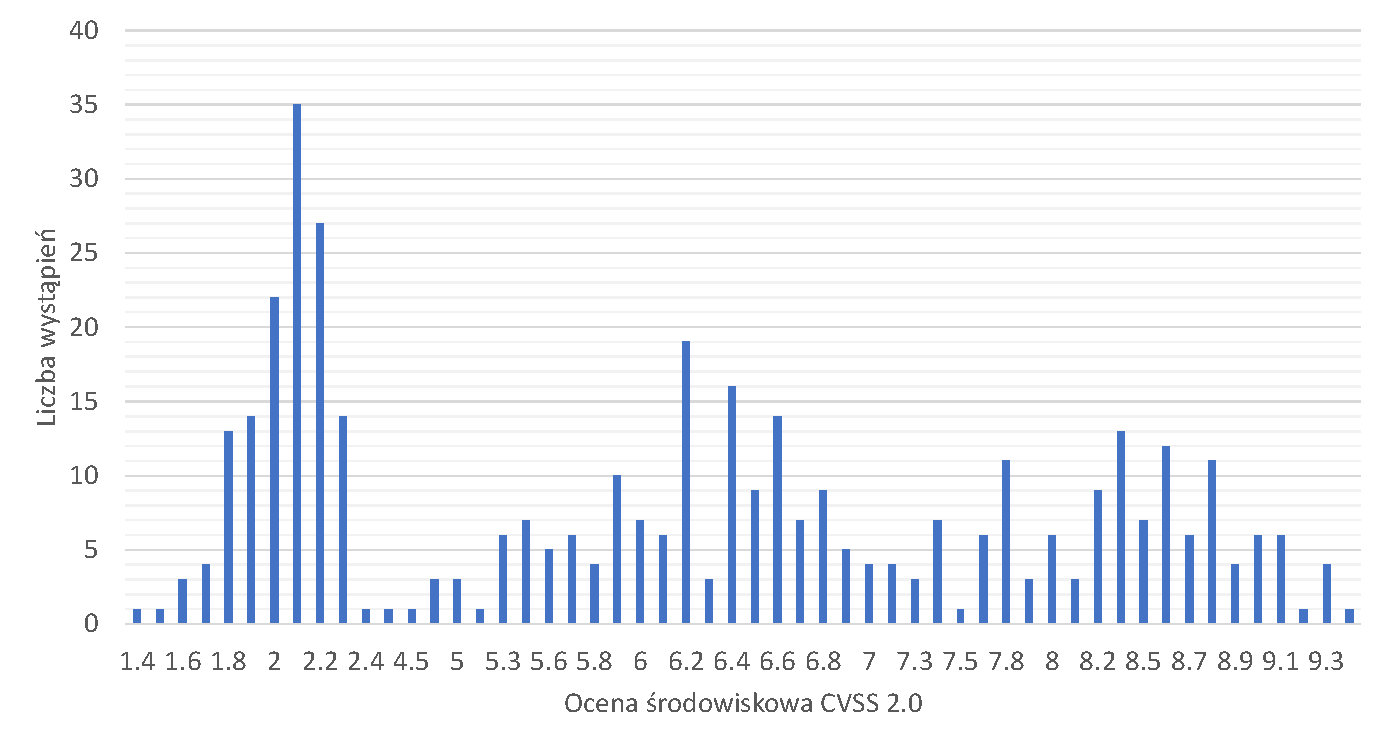
\includegraphics[width=.9\textwidth]{Chapters/Wplyw/cvss2/cvss_2_high.pdf}
\caption{Liczba wystąpień wartości oceny środowiskowej dla różnych ustawień parametrów $CIA$, $CDP$, $TD$ dla oceny bazowej CVSS 2.0 o kategorii wysokiej.}
\label{fig:wplyw:env_a:cvss_2_high}
\end{figure}

\bigbreak
Rysunek \ref{fig:wplyw:env_a:cvss_2_medium} przedstawia liczbę wystąpień wartości oceny środowiskowej dla różnych ustawień parametrów $CIA$, $CDP$, $TD$ dla oceny bazowej CVSS 2.0 o kategorii średniej. Na podstawie wyników przedstawionych na rysunku \ref{fig:wplyw:env_a:cvss_2_medium} można stwierdzić, że dla oceny bazowej CVSS 2.0 o wartości początkowej 4.3 (kategoria średnia) na 540 kombinacji parametrów $CIA$, $CDP$, $TD$ możliwe jest otrzymanie 30 unikalnych wartości oceny środowiskowej CVSS 2.0. Otrzymane wartości oceny środowiskowej CVSS 2.0 mieszczą się w zakresie od 0.8 do 7.7. Z zakresu otrzymanych wartości oceny środowiskowej CVSS 2.0 można wyciągnąć wniosek, że możliwa jest zmiana kategorii krytyczności z średniej na wysoką lub niską. Dla 540 kombinacji parametrów $CIA$, $CDP$, $TD$ dla oceny bazowej CVSS 2.0 o kategorii średniej zmiana jednego parametru środowiskowego może spowodować zmianę kategorii krytyczności na wysoką z prawdopodobieństwem 10.6\%, średnią z prawdopodobieństwem 46.9\% lub niską z prawdopodobieństwem 42.5\%.

\begin{figure}[!ht]
\centering
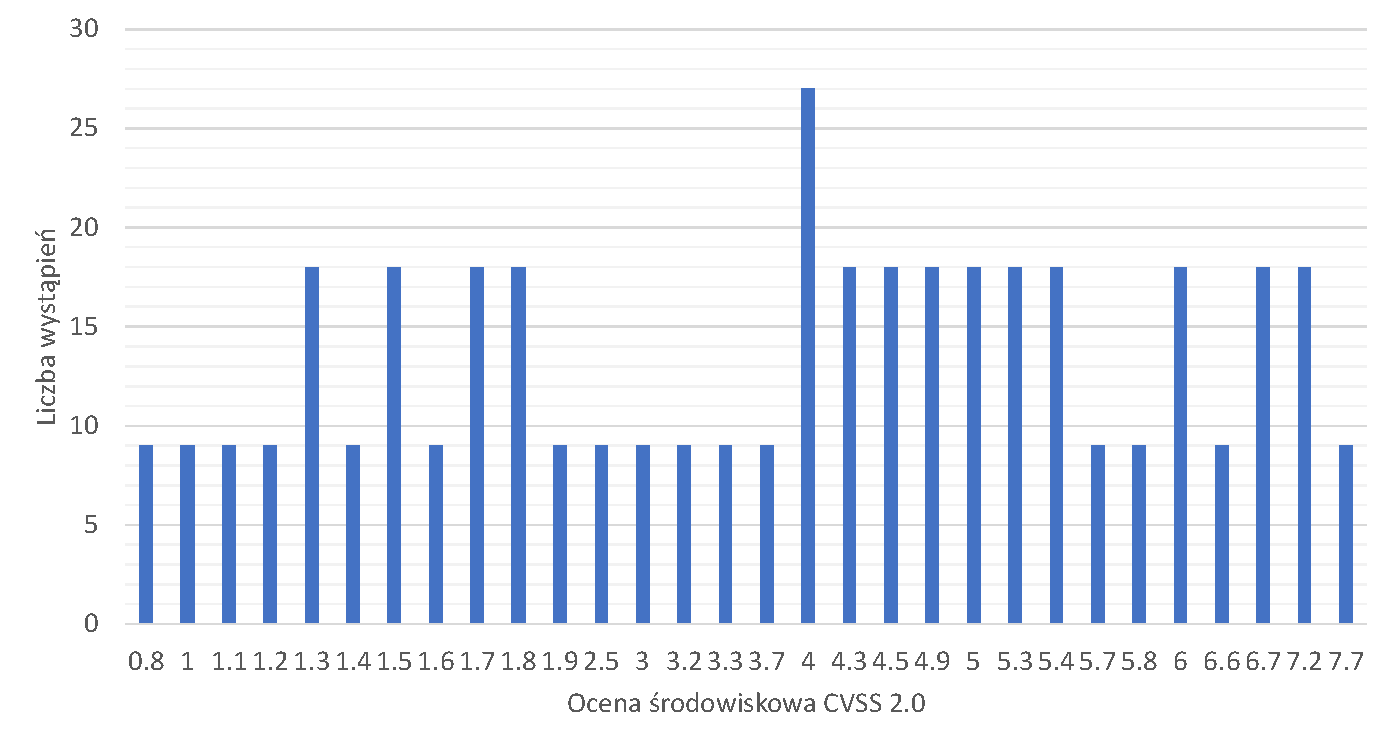
\includegraphics[width=.9\textwidth]{Chapters/Wplyw/cvss2/cvss_2_medium.pdf}
\caption{Liczba wystąpień wartości oceny środowiskowej dla różnych ustawień $CIA$, $CDP$, $TD$ dla oceny bazowej CVSS 2.0 o kategorii średniej.}
\label{fig:wplyw:env_a:cvss_2_medium}
\end{figure}

\bigbreak
Rysunek \ref{fig:wplyw:env_a:cvss_2_low} przedstawia liczbę wystąpień wartości oceny środowiskowej dla różnych ustawień parametrów $CIA$, $CDP$, $TD$ dla oceny bazowej CVSS 2.0 o kategorii niskiej. Na podstawie wyników przedstawionych na rysunku \ref{fig:wplyw:env_a:cvss_2_low} można stwierdzić, że dla oceny bazowej CVSS 2.0 o wartości początkowej 3.3 (kategoria niska) na 540 kombinacji parametrów $CIA$, $CDP$, $TD$ możliwe jest otrzymanie 47 unikalnych wartości oceny środowiskowej CVSS 2.0. Otrzymane wartości oceny środowiskowej CVSS 2.0 mieszczą się w zakresie od 0.4 do 7.4. Z zakresu otrzymanych wartości oceny środowiskowej CVSS 2.0 można wyciągnąć wniosek, że możliwa jest zmiana kategorii krytyczności z niskiej na wysoką lub średnią. Dla 540 kombinacji parametrów $CIA$, $CDP$, $TD$ dla oceny bazowej CVSS 2.0 o kategorii niskiej zmiana jednego parametru środowiskowego może spowodować zmianę kategorii krytyczności na wysoką z prawdopodobieństwem 2.2\%, średnią z prawdopodobieństwem 41.5\% lub niską z prawdopodobieństwem 56.3\%.

\begin{figure}[!ht]
\centering
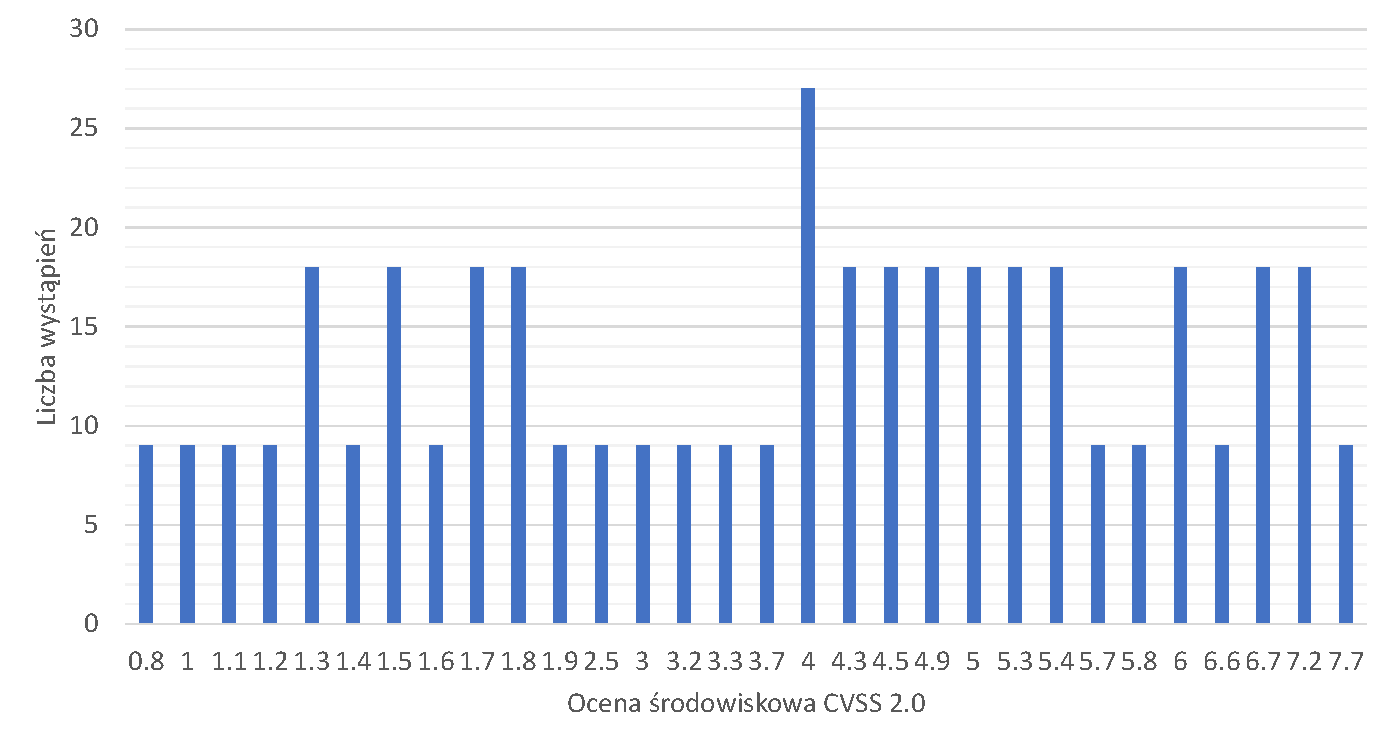
\includegraphics[width=.9\textwidth]{Chapters/Wplyw/cvss2/cvss_2_low.pdf}
\caption{Liczba wystąpień wartości oceny środowiskowej dla różnych ustawień parametrów $CIA$, $CDP$, $TD$ dla oceny bazowej CVSS 2.0 o kategorii niskiej.}
\label{fig:wplyw:env_a:cvss_2_low}
\end{figure}

\bigbreak
Na podstawie analizy wyników stwierdza się znaczący wpływ parametrów środowiskowych $TD$, $CDP$, $CIA$ na ocenę bazową CVSS 2.0. Ich prawidłowy dobór pozwala dopasować ocenę oraz krytyczność do monitorowanego środowiska teleinformatycznego dla wszystkich rozpatrywanych przypadków. Jak wykazano w analizie istnieje, 540 możliwych kombinacji parametrów środowiskowych, co przekłada się na znaczną liczbę unikalnych wartości oceny środowiskowej CVSS 2.0. Dla podatności o kategorii wysokiej z oceną bazową CVSS 2.0 o wartości 7.5 istnieje 55 unikalnych wartości oceny środowiskowej (Rysunek \ref{fig:wplyw:env_a:cvss_2_high}), która umożliwia zmianę kategorii z wysokiej na niską. Dla podatności o kategorii średniej z oceną bazową CVSS 2.0 o wartości 4.3 istnieje 30 unikalnych wartości oceny środowiskowej (Rysunek \ref{fig:wplyw:env_a:cvss_2_medium}), która umożliwia zmianę kategorii z średniej na niską lub wysoką. Dla podatności o kategorii niskiej z oceną bazową CVSS 2.0 o wartości 3.3 analiza wykazała 47 możliwych unikalnych wartości (Rysunek \ref{fig:wplyw:env_a:cvss_2_low}), która umożliwia zmianę kategorii z niskiej na średnią lub wysoką. Na podstawie otrzymanych wyników dotyczących standardu CVSS 2.0 stwierdza się, że parametry środowiskowe $CIA$, $CDP$, $TD$ mają znaczący wpływ na zmianę oceny oraz kategorii podatności. W kolejnym rozdziale przedmiotem analizy są otrzymane wyniki wybranych modeli zarządzania podatnościami wykorzystującymi standard CVSS 2.0 dla trzech niezależnych środowisk teleinformatycznych.

%%%%%%%%%%%%%%%%%%%%%%%%%%%%%%%%%%%%%%%%%%%%%%%%

%%%%%%%%%%%%%%%%%%%%%%%%%%%%%%%%%%%%%%%%%%%%%%%%
\section{Wpływ parametrów środowiskowych na ocenę bazową CVSS 3.x}
\label{sec:wplyw_cvss3}
Tabela \ref{tab:wplyw:env_a:cve_cvss_2} zawiera podatności wykryte w środowisku teleinformatycznym A dla każdej kategorii krytyczności według oceny bazowej CVSS 3.x. Podatności przedstawione w tabeli \ref{tab:wplyw:env_a:cve_cvss_2} zostały wybrane w sposób losowy w celu umożliwienia przeprowadzenia analizy wpływu parametrów $CIA$ na zmianę kategorii krytyczności. W przypadku zastosowania parametrów $CIA$ istnieją 64 możliwe kombinacje parametrów środowiskowych $CIA$. Natomiast według dokumentacji \cite{cvs2019specification} można wykluczyć wartości \emph{Not Defined} (X), ponieważ nie mają one wpływu na ocenę bazową. W związku z czym pozostaje tylko 27 możliwych kombinacji.

\begin{table}[tbh]
\caption{Podatności wykryte w środowisku teleinformatycznym A dla każdej kategorii krytyczności według oceny bazowej CVSS 3.x.}
\begin{center}
\label{tab:wplyw:env_a:cve_cvss_3}
\begin{tabular}{lcl}
\hline \noalign {\smallskip}
\textbf{CVE ID}  & \textbf{Ocena bazowa} & \textbf{Kategoria}  \\
                 & \textbf{CVSS 3.x} &  \\
\hline \noalign {\smallskip}
CVE-2019-13224 & 9.8 & Krytyczna \\
CVE-2020-7062  & 7.5 & Wysoka \\
CVE-2020-7066  & 4.3 & Średnia \\
CVE-2020-7068  & 3.6 & Niska \\
\hline \noalign {\smallskip}
\end{tabular}
\end{center}
\end{table}

\begin{comment}
\bigbreak
Rysunek \ref{fig:wplyw:env_a:cvss_3_distribution} przedstawia wpływ ustawień parametrów środowiskowych $CIA$ na oceny bazowe CVSS 3.x dla podatności wskazanych w tabeli \ref{tab:wplyw:env_a:cve_cvss_3}. Na podstawie wyników przedstawionych na rysunku \ref{fig:wplyw:env_a:cvss_3_distribution} można stwierdzić, że liczba możliwych wartości oceny środowiskowej CVSS 3.x jest bardzo ograniczona w porównaniu do oceny środowiskowej CVSS 2.0. Natomiast nie zmienia to faktu, że każda z przedstawionych podatności za pomocą parametrów $CIA$ może zmienić kategorię krytyczności co zostało potwierdzone w dalszej części analizy.

\begin{figure}[!ht]
\centering
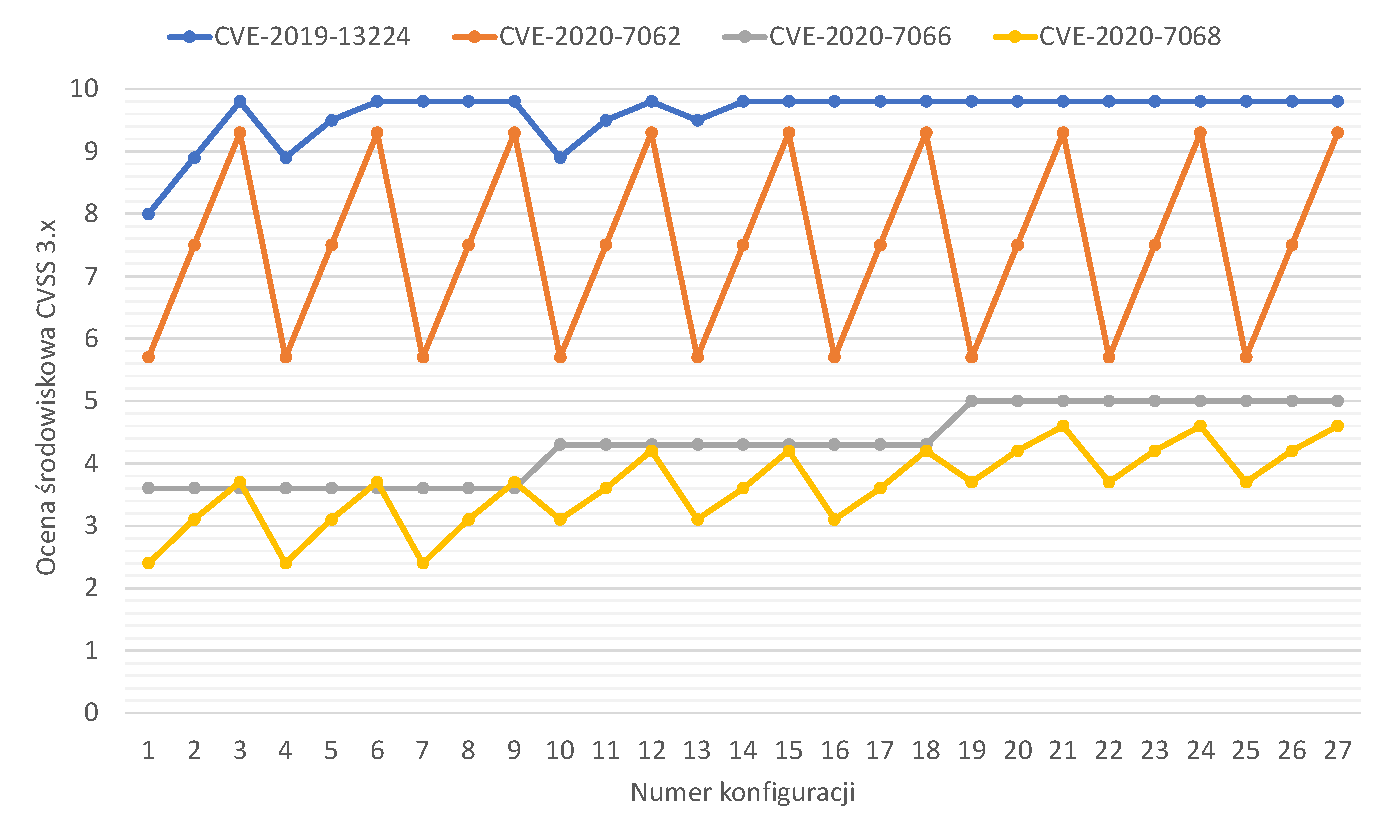
\includegraphics[width=.9\textwidth]{Chapters/Wplyw/cvss3/cvss_3_distribution.pdf}
\caption{Wpływ ustawień parametrów środowiskowych $CIA$ na oceny bazowe CVSS 3.x dla podatności wskazanych w tabeli \ref{tab:wplyw:env_a:cve_cvss_3}.}
\label{fig:wplyw:env_a:cvss_3_distribution}
\end{figure}
\end{comment}

\bigbreak
Rysunek \ref{fig:wplyw:env_a:cvss_3_critical} przedstawia liczbę wystąpień wartości oceny środowiskowej dla różnych ustawień parametrów $CIA$ dla oceny bazowej CVSS 3.x o kategorii krytycznej. Na podstawie wyników przedstawionych na rysunku \ref{fig:wplyw:env_a:cvss_3_critical} można stwierdzić, że dla oceny bazowej CVSS 3.x o wartości początkowej 9.8 (kategoria krytyczna) na 27 kombinacji parametrów $CIA$ otrzymano 4 unikalne wartości oceny środowiskowej CVSS 3.x. Otrzymane wartości oceny środowiskowej CVSS 3.x mieszczą się w zakresie od 8 do 9.8. Z zakresu otrzymanych wartości oceny środowiskowej CVSS 3.x można stwierdzić, że możliwa jest zmiana kategorii z krytyczej na wysoką. Dla 27 kombinacji parametrów $CIA$ dla oceny bazowej CVSS 3.x o kategorii krytycznej zmiana jednego parametru środowiskowego może spowodować zmianę kategorii krytyczności na wysoką z prawdopodobieństwem 3.7\% lub krytyczną z prawdopodobieństwem 96.3\%.

\begin{figure}[!ht]
\centering
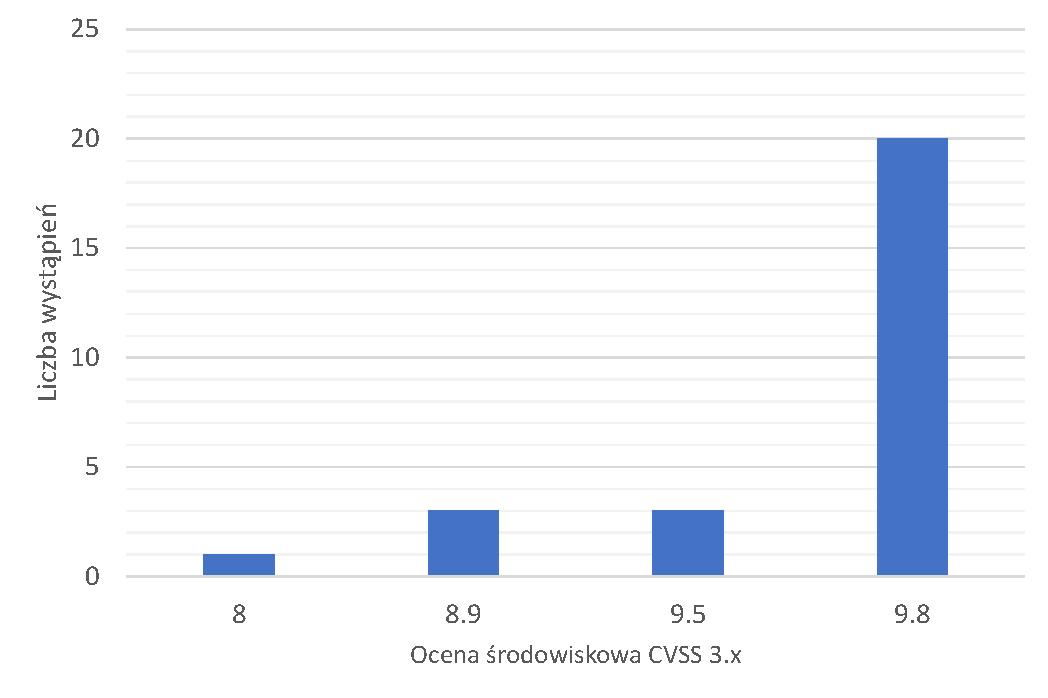
\includegraphics[width=.9\textwidth]{Chapters/Wplyw/cvss3/cvss_3_critical.pdf}
\caption{Liczba wystąpień wartości oceny środowiskowej dla różnych ustawień parametrów $CIA$ dla oceny bazowej CVSS 3.x o kategorii krytycznej.}
\label{fig:wplyw:env_a:cvss_3_critical}
\end{figure}

\bigbreak
Rysunek \ref{fig:wplyw:env_a:cvss_3_high} przedstawia liczbę wystąpień wartości oceny środowiskowej dla różnych ustawień parametrów $CIA$ dla oceny bazowej CVSS 3.x o kategorii wysokiej. Na podstawie wyników przedstawionych na rysunku \ref{fig:wplyw:env_a:cvss_3_high} można stwierdzić, że dla oceny bazowej CVSS 3.x o wartości początkowej 7.5 (kategoria wysoka) na 27 kombinacji parametrów $CIA$ otrzymano tylko 3 unikalne wartości oceny środowiskowej CVSS 3.x. Otrzymane wartości oceny środowiskowej CVSS 3.x mieszczą się w zakresie od 5.7 do 9.3. Z zakresu otrzymanych wartości oceny środowiskowej CVSS 3.x można stwierdzić, że możliwa jest zmiana kategorii z wysokiej na średnią lub krytyczną. Dla 27 kombinacji parametrów $CIA$ dla oceny bazowej CVSS 3.x o kategorii wysokiej zmiana jednego parametru środowiskowego może spowodować zmianę kategorii krytyczności na krytyczną z prawdopodobieństwem 33.(3)\%, średnią z prawdopodobieństwem 33.(3)\% lub wysoką z prawdopodobieństwem 33.(3)\%.

\begin{figure}[!ht]
\centering
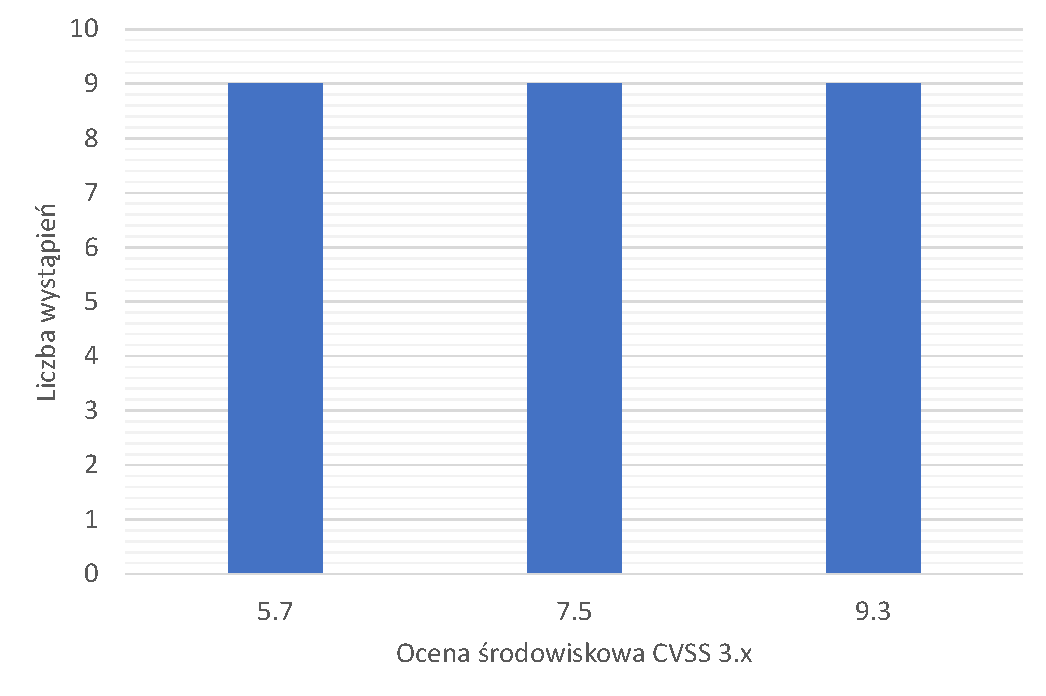
\includegraphics[width=.9\textwidth]{Chapters/Wplyw/cvss3/cvss_3_high.pdf}
\caption{Liczba wystąpień wartości oceny środowiskowej dla różnych ustawień parametrów $CIA$ dla oceny bazowej CVSS 3.x o kategorii wysokiej.}
\label{fig:wplyw:env_a:cvss_3_high}
\end{figure}

\bigbreak
Rysunek \ref{fig:wplyw:env_a:cvss_3_medium} przedstawia liczbę wystąpień wartości oceny środowiskowej dla różnych ustawień parametrów $CIA$ dla oceny bazowej CVSS 3.x o kategorii średniej. Na podstawie wyników przedstawionych na rysunku \ref{fig:wplyw:env_a:cvss_3_medium} można stwierdzić, że dla oceny bazowej CVSS 3.x o wartości początkowej 4.3 (kategoria średnia) na 27 kombinacji parametrów $CIA$ otrzymano tylko 3 unikalne wartości oceny środowiskowej CVSS 3.x. Otrzymane wartości oceny środowiskowej CVSS 3.x mieszczą się w zakresie od 3.6 do 5.0. Z zakresu otrzymanych wartości oceny środowiskowej CVSS 3.x można stwierdzić, że możliwa jest zmiana kategorii z średniej na niską. Dla 27 kombinacji parametrów $CIA$ dla oceny bazowej CVSS 3.x o kategorii wysokiej, zmiana jednego parametru środowiskowego może spowodować zmianę kategorii krytyczności na średnią z prawdopodobieństwem 66.(6)\% lub niską z prawdopodobieństwem 33.(3)\%.

\begin{figure}[!ht]
\centering
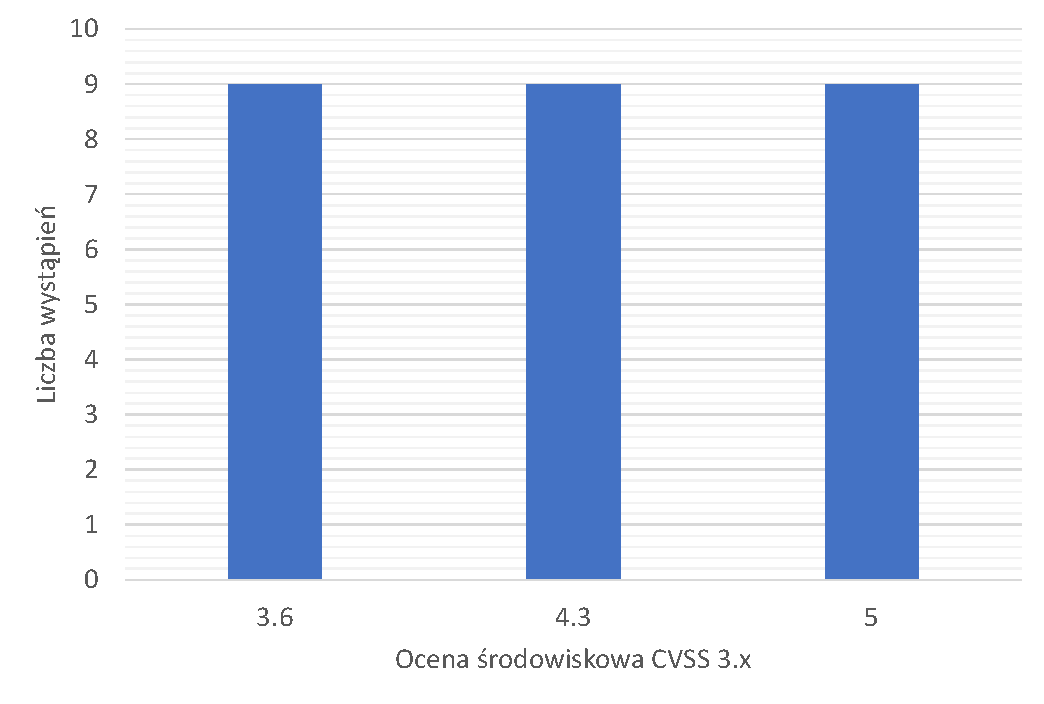
\includegraphics[width=.9\textwidth]{Chapters/Wplyw/cvss3/cvss_3_medium.pdf}
\caption{Liczba wystąpień wartości oceny środowiskowej dla różnych ustawień parametrów $CIA$ dla oceny bazowej CVSS 3.x o kategorii średniej.}
\label{fig:wplyw:env_a:cvss_3_medium}
\end{figure}

\bigbreak
Rysunek \ref{fig:wplyw:env_a:cvss_3_low} przedstawia liczbę wystąpień wartości oceny środowiskowej dla różnych ustawień parametrów $CIA$ dla oceny bazowej CVSS 3.x o kategorii niskiej. Na podstawie wyników przedstawionych na rysunku \ref{fig:wplyw:env_a:cvss_3_low} można stwierdzić, że dla oceny bazowej CVSS 3.x o wartości początkowej 3.6 (kategoria niska) na 27 kombinacji parametrów $CIA$ otrzymano 6 unikalnych wartości oceny środowiskowej CVSS 3.x. Otrzymane wartości oceny środowiskowej CVSS 3.x mieszczą się w zakresie od 2.4 do 4.6. Z zakresu otrzymanych wartości oceny środowiskowej CVSS 3.x można stwierdzić, że możliwa jest zmiana kategorii z niskiej na średnią. Dla 27 kombinacji parametrów $CIA$ dla oceny bazowej CVSS 3.x o kategorii niskiej zmiana jednego parametru środowiskowego może spowodować zmianę kategorii krytyczności na niską z prawdopodobieństwem 66.(6)\% lub średnią z prawdopodobieństwem 33.(3)\%.

\begin{figure}[!ht]
\centering
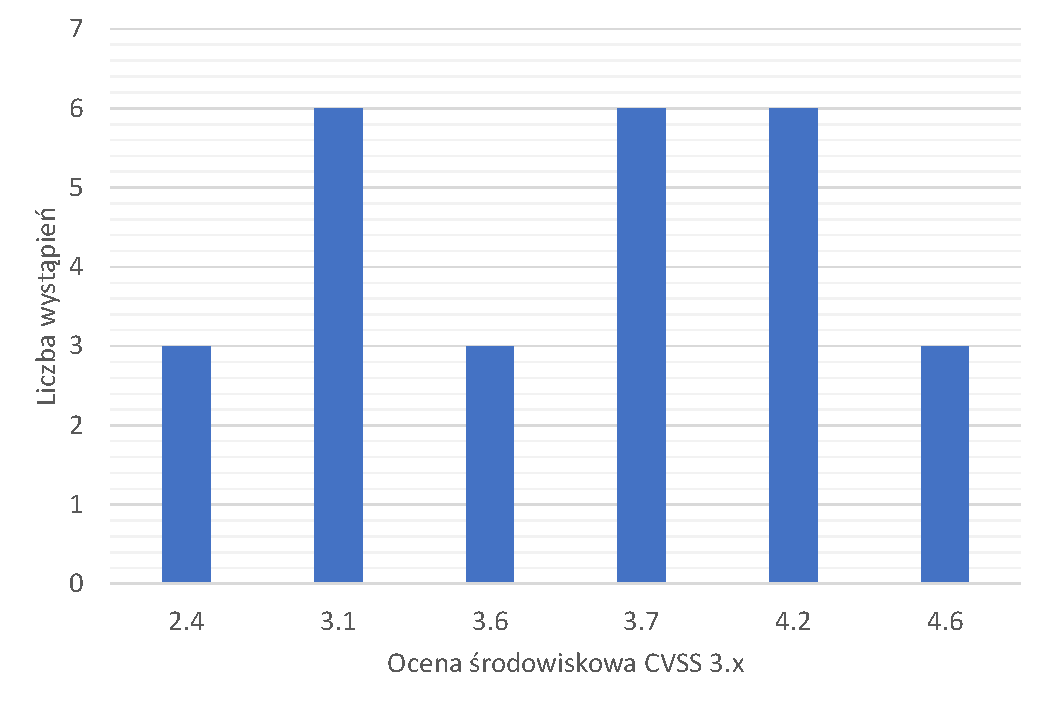
\includegraphics[width=.9\textwidth]{Chapters/Wplyw/cvss3/cvss_3_low.pdf}
\caption{Liczba wystąpień wartości oceny środowiskowej dla różnych ustawień parametrów $CIA$ dla oceny bazowej CVSS 3.x o kategorii niskiej.}
\label{fig:wplyw:env_a:cvss_3_low}
\end{figure}

\bigbreak
Na podstawie analizy wyników stwierdza się znaczący wpływ parametrów środowiskowych $CIA$ na ocenę bazową CVSS 3.x. Otrzymane wyniki potwierdzają, że prawidłowy dobór parametrów środowiskowych $CIA$ pozwala dopasować ocenę oraz kategorię do monitorowanego środowiska teleinformatycznego. Jak wykazano w analizie, istnieje 27 możliwych kombinacji wartości parametrów środowiskowych $CIA$, które mogą zmieniać kategorię krytyczności podatności. Dla podatności o kategorii wysokiej z oceną bazową CVSS 3.x wynoszącą 9.8 istnieją 4 możliwe unikalne wartości oceny środowiskowej (Rysunek \ref{fig:wplyw:env_a:cvss_3_critical}), które umożliwiają zmianę kategorii tylko z krytycznej na wysoką. Dla podatności o kategorii wysokiej z oceną bazową CVSS 3.x wynoszącą 7.5, istnieją tylko 3 możliwe unikalne wartości oceny środowiskowej, które umożliwiają zmianę kategorii z wysokiej na średnią lub krytyczną. Dla podatności o kategorii średniej z oceną bazową CVSS 3.x wynoszącą 4.3 istnieją 3 możliwe unikalne wartości oceny środowiskowej, które pozwalają na zmianę kategorii krytyczności z średniej na niską. Dla podatności o kategorii niskiej z oceną bazową CVSS 3.x wynoszącą 3.6 istnieje 6 możliwych unikalnych wartości oceny środowiskowej, dzięki którym możliwa jest zmiana kategorii z niskiej na średnią. Na podstawie otrzymanych wyników dotyczących standardu CVSS 3.x stwierdza się, że parametry środowiskowe $CIA$ mają znaczący wpływ na zmianę oceny oraz kategorii podatności. W kolejnym rozdziale przedmiotem analizy są otrzymane wyniki wybranych modeli zarządzania podatnościami wykorzystującymi standard CVSS 3.x dla trzech niezależnych środowisk teleinformatycznych.

%%%%%%%%%%%%%%%%%%%%%%%%%%%%%%%%%%%%%%%%%%%%%%%%

%%%%%%%%%%%%%%%%%%%%%%%%%%%%%%%%%%%%%%%%%%%%%%%%
\section{Wyniki analizy metod konwersji oceny bazowej CVSS 2.0 do 3.x}
\label{sec:ml_analiza}

Tabela \ref{tab2} przedstawia wybrane algorytmy klasyfikacji z uwzględnieniem liczby PC i liczby elementów wektora uczącego do określenia parametrów oceny bazowej CVSS 3.x.
Tabela \ref{tab2} zawiera informacje, przy której wartości PC  i dla jakiej liczby dodatkowych elementów wektora oceny bazowej CVSS 2.0 uzyskano wysoką i powtarzalną wartość skuteczności klasyfikacji. Dla parametrów opisanych w tabeli \ref{tab2}, zbiór uczący składał się z 1 968 wektorów.


\begin{table}[htbp]
\caption{Wybrane algorytmy klasyfikacji, z uwzględnieniem liczby PC i liczby elementów wektora uczącego do określenia parametrów oceny bazowej CVSS 3.x.}
\begin{center}
\begin{tabular}{cccc}
\hline
\textbf{Parametr oceny} & \textbf{Algorytm}   & \textbf{Liczba}  & \textbf{Liczba elementów}  \\
\textbf{bazowej CVSS 3.x}  &             & \textbf{PC}    & \textbf{wektora}    \\
\hline
AV           & KSVM(TGRBF)    & 35     & 100   \\
AC           & PNN            & 25     & 100   \\
PR           & KSVM(TGRBF)    & 24     & 50    \\
U            & PNN            & 41     & 100   \\
C            & KSVM(TGRBF)    & 43     & 50    \\
I            & KSVM(TGRBF)    & 32     & 100   \\
A            & PNN            & 48     & 100   \\
S            & NB             & 38     & 100   \\
\hline
\end{tabular}
\label{tab2}
\end{center}
\end{table}

\bigbreak
Rysunek \ref{fig:wplyw:ml:fig_1} przedstawia średnią dokładność klasyfikacji parametrów wektora oceny bazowej CVSS 3.x za pomocą algorytmów przedstawionych w tabeli \ref{tab2}. Wyniki ukazane na rysunku \ref{fig:wplyw:ml:fig_1} zostały obliczone na podstawie wykonania dziesięciu prób testowych na 71 000 losowo wybranych wektorach. Dokładność obliczono, sumując liczbę poprawnych klasyfikacji i dzieląc przez liczbę wszystkich wektorów testujących. Wyniki przedstawione na rysunku \ref{fig:wplyw:ml:fig_1} pokazują, że dla wszystkich parametrów mediana skuteczności klasyfikacji przekracza 90\%. Uzyskane wyniki są bardzo powtarzalne, poza parametrami AV i PR. W przypadku AV rozpiętości są większe, ale minimalna wartość dokładności wynosi 88,2\%. Prawidłowa klasyfikacja AV z wersji oceny bazowej CVSS 2.0 do 3.x jest utrudniona ze względu na różnicę w standardach CVSS. W przypadku klasyfikacji PR wystąpiły 2 wartości odstające, z wartością minimalną 87,81 \%. Przy obliczaniu zakresu najlepszy okazuje się algorytm NB (mediana to 94,86\%). Bardziej zaawansowane metody są o kilka punktów procentowych gorsze. Parametry AC, U i A były bardzo dobrze konwertowane przez PNN, która dodatkowo należy do algorytmów szybkiego uczenia. W najtrudniejszych przypadkach – AV, PR, C i I najlepszą skuteczność rozpoznawania zapewnia SVM TGRBF. Stopień złożoności tego algorytmu przekłada się na wydłużony czas przetwarzania w porównaniu z innymi algorytmami.

\begin{figure}[!ht]
\centering
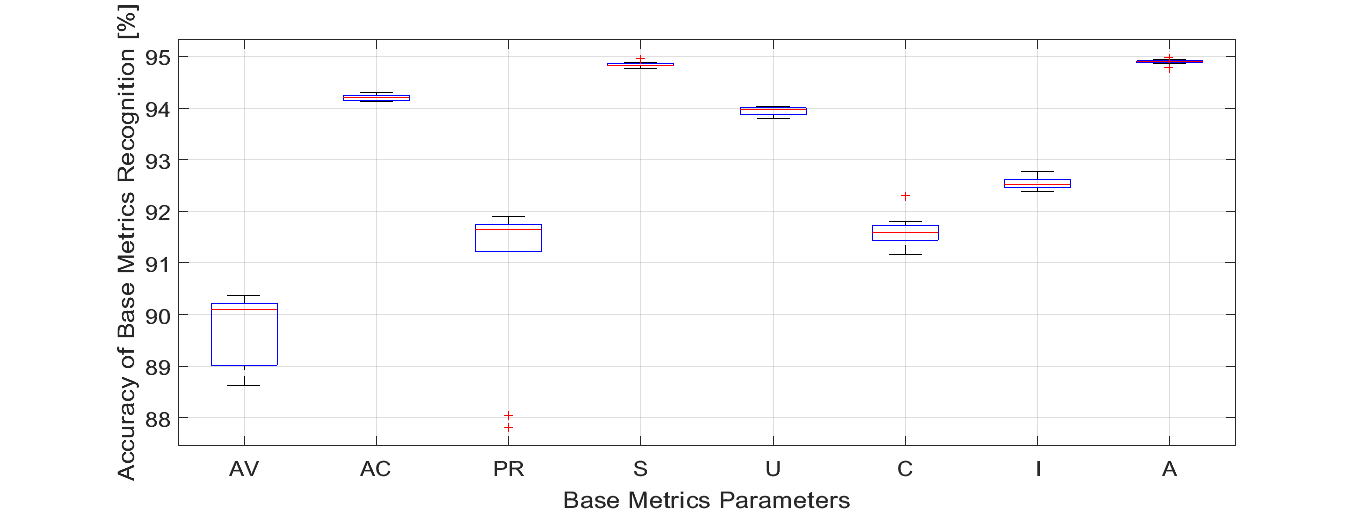
\includegraphics[width=0.95\textwidth]{Chapters/Wplyw/ml_results/Param_Limit_71000_multi_10.png}
\caption{Statystyka dokładność klasyfikacji parametrów wektora oceny bazowej CVSS 3.x za pomocą programu algorytmów przedstawionych tabeli \ref{tab2}.}
\label{fig:wplyw:ml:fig_1}
\end{figure}

\bigbreak
Tabela \ref{tab3} przedstawia medianę i średnią dokładność obliczoną dla algorytmów przedstawionych w tabeli \ref{tab2}. Wyniki przedstawione w tabeli \ref{tab3} zostały uzyskane z 10 krotnej próby testowej algorytmów z losowo wybranym 71 000 zbiorem testowym. Na podstawie wyników przedstawionych w tabeli \ref{tab3} można stwierdzić, że poza AV i PR wykazują niewielkie odchylenie standardowe od średniej, a wartości średnie różnią się od mediany maksymalnie o 0,07\%. Otrzymane wyniki potwierdzają wysoką precyzję określania parametrów oceny bazowej CVSS 3.x przez wybrane algorytmy.

\begin{table}[htbp]
\caption{Mediana i średnia dokładność obliczona dla algorytmów przedstawionych w tabeli \ref{tab2}.}
\begin{center}
\begin{tabular}{cccc}
\hline
\textbf{Parametr oceny} & \textbf{Mediana [\%]}   & \textbf{Średnia [\%]}  \\
\textbf{bazowej CVSS 3.x} & & \\
\hline
AV           & 90.10    & $89.73\pm0.66$     \\
AC           & 94.21    & $94.21\pm0.06$     \\
PR           & 91.64    & $90.89\pm1.49$     \\
S            & 94.86    & $94.84\pm0.05$     \\
U            & 94.02    & $93.95\pm0.07$     \\
C            & 91.59    & $91.62\pm0.29$     \\
I            & 92.51    & $92.53\pm0.11$     \\
A            & 94.94    & $94.90\pm0.05$     \\
\hline
\end{tabular}
\label{tab3}
\end{center}
\end{table}

\bigbreak
Rysunek \ref{fig:wplyw:ml:qsrs_base_score} przedstawia macierz błędów klasyfikacji kategorii podatności z oceny bazowej CVSS 2.0 do 3.x. Wyniki przedstawione na rysunku \ref{fig:wplyw:ml:qsrs_base_score} zostały uzyskane dla 71 000 podatności pobranych z serwisu NVD \cite{booth2013national}. Na rysunku \ref{fig:wplyw:ml:qsrs_base_score} klasa 0 oznacza podatność o klasyfikacji informacyjnej; 1 - niskiej; 2 - średniej; 3 - wysokiej; oraz 4 - krytycznej. Na podstawie wyników przedstawionych na rysunku \ref{fig:wplyw:ml:qsrs_base_score} można stwierdzić, że zastosowane rozwiązanie najlepiej radzi sobie z klasyfikacją oceny bazowej CVSS 3.x dla kategorii krytycznej (precyzja 90.3\%, czułość 87.8\%), a najgorzej z klasyfikacją dla kategorii niskiej (precyzja 27\%, czułość 12.4\%). Dodatkowo na podstawie wyników przedstawionych na rysunku \ref{fig:wplyw:ml:qsrs_base_score} można stwierdzić, że średnia sprawność dla klasyfikacji wszystkich kategorii wynosi 86\%.

\begin{figure}[!ht]
\centering
\includegraphics[width=0.95\textwidth]{Chapters/Wplyw/ml_results/Macierz_błędów_QSRS.png}
\caption{Macierz błędów klasyfikacji kategorii podatności z oceny bazowej CVSS 2.0 do 3.x.}
\label{fig:wplyw:ml:qsrs_base_score}
\end{figure}

\bigbreak
Na podstawie uzyskanych wyników stwierdza się, że zaproponowane algorytmy uczenia maszynowego wykorzystane do konwersji oceny bazowej CVSS 2.0 do 3.x wykazują wysoką skuteczność wyznaczania podstawowych parametrów wektora oceny bazowej CVSS 3.x. Otrzymana mediana dla najgorszego rozpatrywanego przypadku, tj. dla parametru AV, przekracza 90\%. Na podstawie otrzymanych wyników można stwierdzić, że sprawność obliczania oceny bazowej CVSS 3.x wynosi 62.8\%, natomiast średnia sprawność klasyfikacji dla wszystkich kategorii krytyczności wynosi 86\%.
